\chapter{Bose-Einstein condensation in complex networks}

\section{Fitnes model and Bose gas mapping}
 

%In complex sistems, different nodes compete to attract new links generated by new nodes entering the network. Examples are the World Wide Web, where webpages compete for URLs to increase their visibility; the citation network of scientific pubblications, where the oldest and most important papers are the most cited; companies try to attract more customers. All the nodes in these networks tend to acquire more links than the other nodes based on two features: their \emph{fitness}, a measure of the goodness of the node itself (a revolutionary paper, a company's successfull product) and the number of links...........


The \emph{fitness model} introduced in \cite{ba2000competition} describes a system where the nodes with more links or greater fitness (a measure of their ability to attract new edges) are more likely to make new conncections over time. The model reproduces the behaviour of companies, trying to acquire new customers, or the network of scientific papers, where articles try to acquire new citations. The network is generated as follows: at each time step, a new node is added and $m$ new links are formed, from the new node to the old ones. Each new node $i$ has a fitness value $\eta_i$, sampled from the distribution $\rho(\eta)$ the new node connects  one of its links to node $j$ in the network with probability $\Pi_j$ defined as 

\begin{equation}
    \Pi_j = \frac{\eta_j \; k_j}{\sum_q \eta_q\; k_q}
\end{equation}

Thus, nodes with larger fitness and higher degree are more likely to acquire new links. Older nodes are more favoured, since they immediately make new connections and increase their degree, but a new node with large fitness, introduced at later time, can still compete.

It has been shown in \cite{ba2001bose-einstein} that the fitness model can undergo a phase transition, analog to a Bose-Einstein condensation. To construct the Bose gas, the energy levels are mapped as follows

\begin{equation}
    \epsilon_i = - \frac{1}{\beta} \log \eta_i
\end{equation}

where $\beta = 1/T$ is the inverse temperature.
It can be shown that the chemical potential defined as 

\begin{equation}\label{eq:zt}
    e^{-\beta \mu } = \lim_{t\to \infty} \frac{Z_t}{mt}  ,
\end{equation}

where $ Z_t = \sum_q \eta_q\; k_q(t)$ is the partition function, is the solution of 

\begin{equation}
      I(\beta, \mu) = \int \dd \epsilon \frac{g(\epsilon)}{e^{\beta(\epsilon-\mu)}-1} = 1
\end{equation}


The integral gives the number of particles of a Bose gas in the thermodynamic limit and volume $v=1$. Being $I(\beta, \mu) \leq \max{I(\beta, \mu)} = I(\beta, 0)$, if $I(\beta, 0) <1$ there is no value of $\mu$ satisfying the above equation: this is a sign of a Bose-Einstein condensate. In this phase, a finite fraction of particles is in the ground state, corresponding to the fittest node. We simulate the growth of a \emph{fitness-model} and show the presence of a phase transition.

\section{Implementation}
We implemented the fitness model described in the previous section and the other analysis in \emph{R}. Following \cite{ba2001bose-einstein}, we chose an exponential energy distribution 

\begin{eqnarray}
    g(\epsilon) = C \epsilon^\theta \quad \epsilon \in [0, \epsilon_{max}]
\end{eqnarray}

where $C=(\theta+1)/\epsilon_{max}^{\theta+1}$ is the normalizing constant.

\begin{figure}[h!]
    \centering
    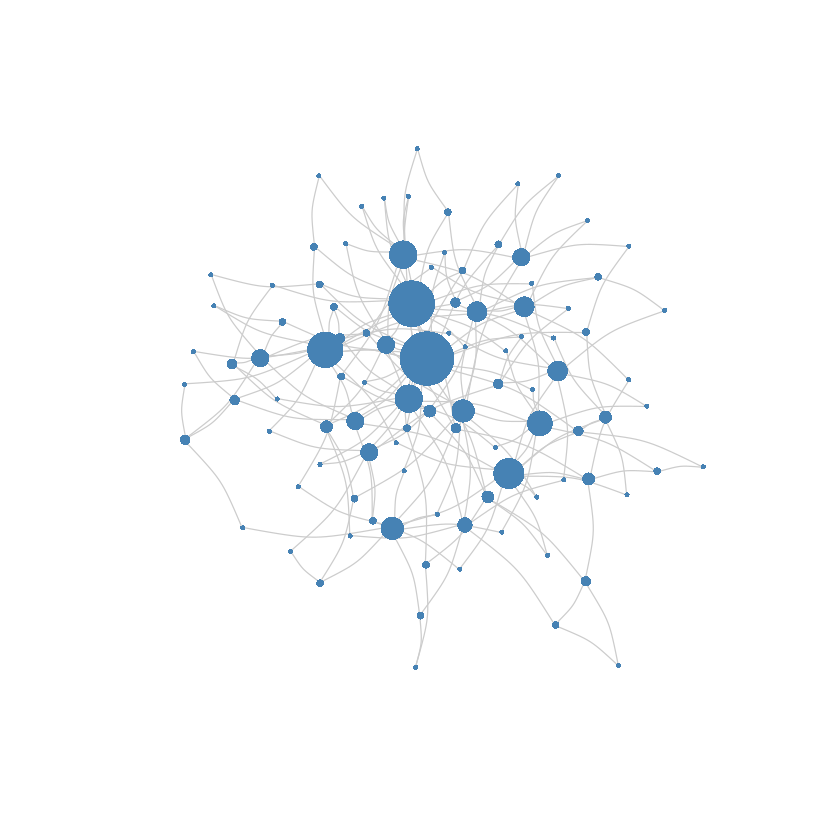
\includegraphics[width=0.7\textwidth]{images/fitness_network.png}
    \label{}
    \caption{Example of fitness model generated with 100 nodes. The size fo each node is proportional to their degree.}
\end{figure}


We simulated the network growth for two different times (sistem sizes) $t=10^3$ and $t=10^4$  at 50 different values of $T$ in the range $[0.03, 10]$.  We didn't simulate the system for $t=10^5$, as in \cite{ba2001bose-einstein}, due to excessive computing time.
For each value of $T$ we ran  $M=80$  (for $t=10^3$) and $M=50$ (for $t=10^4$) independent simulations of the network to compute statistical averages. Using $\theta=1$ and $\epsilon_{max}=1$, we computed $Z_t$ as in equation \eqref{eq:averages} on the state of the network at time $t$ and then obtained the value of $\mu$ from \eqref{eq:zt}.

\begin{eqnarray}\label{eq:averages}
    <Z_t> = \frac{1}{M} \sum_{runs} Z_t
\end{eqnarray}

Since the simulations are independent, they are run in parallel on each core of a CPU thanks to the \verb|parallel| library, saving computation time.

\begin{figure}[ht] 
    \centering
    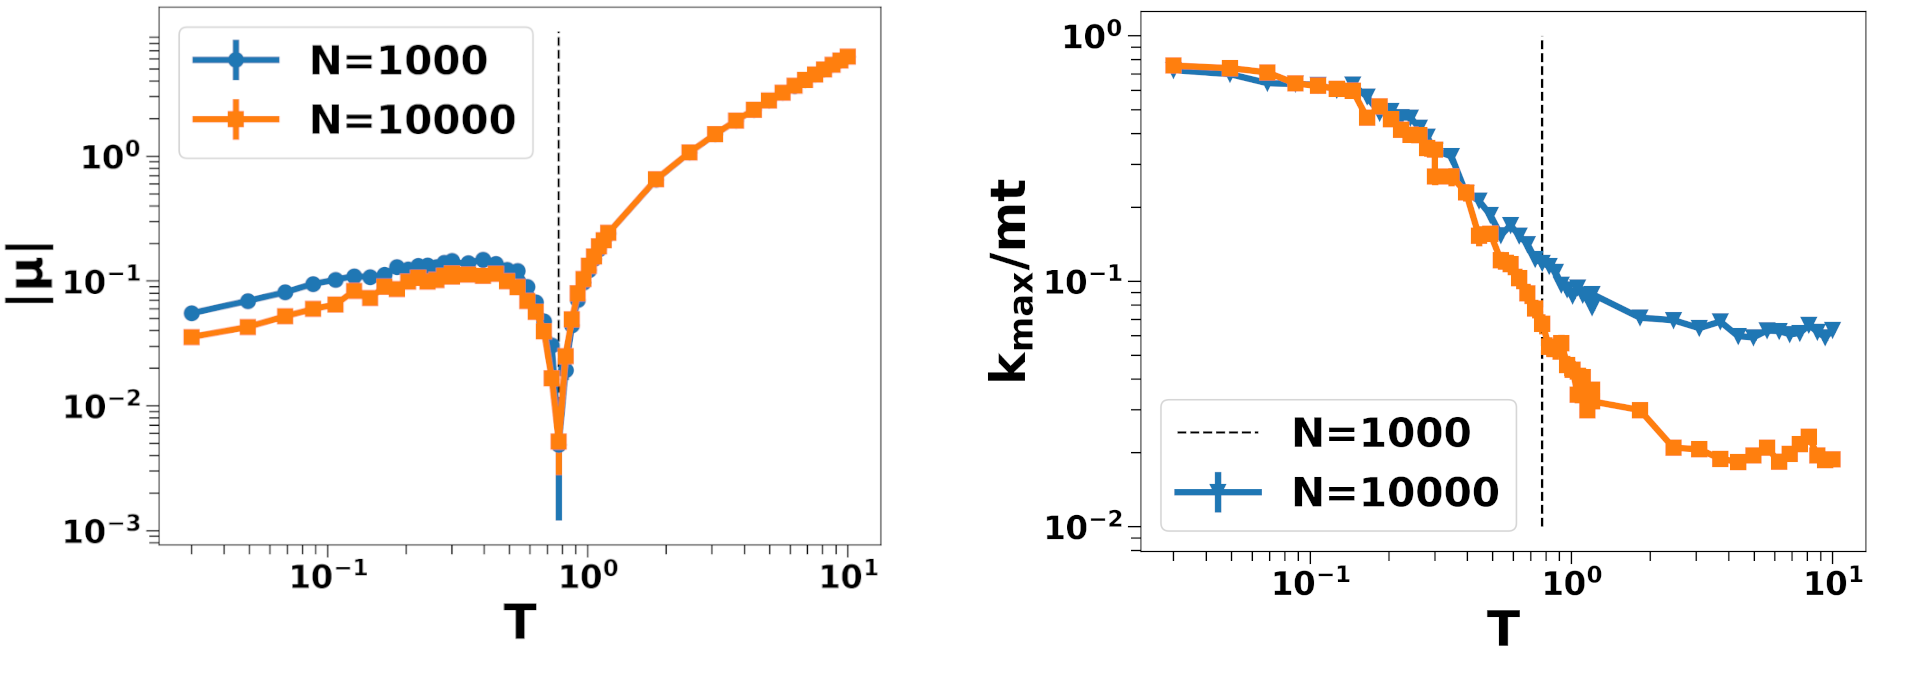
\includegraphics[width=\textwidth]{images/mu_and_gcc.png}
    \caption{Error bars are computed over multiple runs are plotted, but not visible, and $N$ is the number of nodes. Left: the parameter $\mu$ has a quick transition from a positive to negative value, indicating a phase transition. Right: fraction of edges belonging to most connected node as function of $T$.}
    \label{fig:mu}
\end{figure}

In figure \ref{fig:mu} (left), we report the value of $|\mu|$ as a function of $T$ the two system sizes. The chemical potensial shows a sharp transition from a positive to a negative value at the critical temperature $T_c$, marked by the dotted black line (   $\mu$ is negative for $T>T_c$ ). This is a phase transition with order parameter $\mu$.

In figure \ref{fig:mu} (right), we can see the relative size $f=k_{max}/(mt)$ of the highest degree node. For $T<T_c$, this node has a finite fraction of all the edges, showing the Bose-Einstein condensate. Over time, the systems mantains a finite fraction of the nodes. Instead For $T>T_c$, the system is in the \emph{fit-get-rich} phase, when the fitter nodes acquire new links at a higher rate than the others \cite{ba2001bose-einstein} but, as time increases, $f$ decreases and in the thermodynamic limit we have $f\to 0$.

\newpage